\documentclass[12pt]{article}

\author{Tom Hubrecht}
\title{Transmission d'informations entre la Terre et les sondes spatiales}
\date{Juin 2019}

\usepackage[utf8]{inputenc}
\usepackage[left=2cm, right=2cm, top=2cm, bottom=2cm]{geometry}
\usepackage{lmodern}
\usepackage{graphicx}
\usepackage{tikz}
\usepackage{float}

\usepackage[fleqn]{amsmath}
\usepackage{amssymb}

\usepackage{csquotes}
\usepackage[backend=biber, style=numeric, citestyle=verbose, sorting=nyt]{biblatex}
\usepackage[french]{babel}
\usepackage{hyperref}

\usetikzlibrary{shapes,arrows}

\graphicspath{{./Images/}}

%% Include the bibliography %%
\addbibresource{Bibliography.bib}

% Definition of blocks:
\tikzset{%
	block/.style    	= {draw, thick, rectangle, minimum height = 3em, minimum width = 3em},
	rsc/.style			= {draw, thick, rectangle, minimum height = 3em, minimum width = 4em},
	smallblock/.style 	= {draw, thick, rectangle, minimum height = 1em, minimum width = 1em, node distance = 2cm},
	sum/.style      	= {draw, circle, node distance = 1.5cm}, % Adder
	input/.style    	= {coordinate}, % Input
	output/.style   	= {coordinate} % Output
}

%Defining string as labels of certain blocks.
\newcommand{\inpt}{$\boldsymbol{\circ}$}


\begin{document}
\maketitle


\section{Introduction}
L'exploration spatiale est un domaine majeur et actuel de la recherche scientifique, les sondes envoyées ne pouvant souvent pas revenir sur Terre, il est crucial de recevoir les informations récoltées, ce qui me semble être un des aspects les plus intéressants de ce domaine. Les liaisons entre les sondes spatiales et la Terre établissent le transport d'instructions de la Terre vers la sonde ainsi que la transmission en retour des données obtenues par la sonde.


\section{Probl\'ematique}
La r\'eception correcte des informations transmises par une sonde spatiale est conditionn\'ee par le codage des donn\'ees de telle sorte que l'on puisse n\'egliger le bruit occasion\'e par la transmission du message \`a travers l'espace. Puisque plusieurs m\'ethodes de codage ainsi que diff\'erentes mani\`eres de d\'ecoder les messages re\c{c}us sont en concurrence, il faut donc \'etudier le fonctionnement des ces algorithmes ainsi que de les impl\'ementer pour tester leurs performances dans une simulation.


\section{Mod\'elisation d'une transmission dans l'espace}
Le processus de la transmission d'information a \'et\'e mod\'elis\'ee par C. Shannon et prend la forme de la Figure-\ref{fig:shannon}
Dans le cas d'une transmission Sonde-Terre, la source mod\'elise les instruments de mesure et l'\'emetteur repr\'esente le circuit \'emetteur de la sonde. Le r\'ecepteur est une parabole sur la Terre par exemple. Le canal de transmission est le vide de l'espace, on consid\`ere en effet qu'aucun obstacle ne perturbe le signal envoy\'e par la sonde. Ainsi, la source de bruit perturbant le signal produit un bruit blanc additif, ce qui donne un canal de propagation gaussien.


\section{Codes correcteurs d'erreurs}
Pour contrer l'action du bruit lors de la transmission d'informations dans l'espace, il convient de coder le message de telle sorte que l'on puisse r\'ecup\'erer le message originel malgr\'e des erreurs dans le message re\c{c}u.


\subsection{Plusieurs classes de codes}
De nombreux types de codes sont utilis\'es dans les transmission spatiales, tels les Turbocodes ou les codes LDPC (Low-Density Parity Checks) dont l'usage est pr\'econis\'e par le CCSDS, l'organisme proc\'edant \`a la mise en place des standards de t\'el\'ecommunications spatiales, cependant leur principe de fonctionnement est fondamentalement diff\'erent.


\subsection{Turbocodes}
Invent\'es par l'\'equipe de C. Berrou vers 1993, les Turbocodes utilisent deux codages par convolution, l'un portant sur le message \`a envoyer, l'autre sur une permutation al\'eatoire de ce message pour r\'eduire les effets d'un ph\'enom\`ene causant une concentration d'erreurs sur une p\'eriode r\'eduite.


\subsubsection{Codage d'un message}
Le message \`a envoyer est la suite de bool\'eens $(d_k)_{k \in [\![1, N]\!]}$, le codage retourne trois suites de bool\'eens\ref{fig:turbo}, $(X_k)_{k \in [\![1, N]\!]}$, $(Y_{1,k})_{k \in [\![1, N]\!]}$ et $(Y_{2,k})_{k \in [\![1, N]\!]}$ avec $\forall k \in [\![1, N]\!], X_k = d_k$.\\
Les composants Enc sur la figure sont des codeurs convolutifs de la forme Figure-\ref{fig:enc}
L'\'etat interne $(M_1, M_2, M_3, M_4)$ du codeur peut \^etre repr\'esent\'e par un entier $S \in [\![0, 15]\!]$, l'entier $K = 4$ est le nombre de cases m\'emoires du composant codeur.


\subsubsection{D\'ecodage du signal re\c{c}u}
Le signal re\c{c}u est ensuite compos\'ee de trois suites de variables r\'eelles $(x_k)_{k \in [\![1, N]\!]}$, $(y_{1,k})_{k \in [\![1, N]\!]}$ et $(y_{2,k})_{k \in [\![1, N]\!]}$ telles que :
\begin{align*} \label{dec_input}
	x_k & = (2.X_k - 1) + a_k \\
	y_{1,k} & = (2.Y_{1,k} - 1) + b_k \\
	y_{2,k} & = (2.Y_{2,k} - 1) + c_k
\end{align*}
o\`u $a_k, b_k$ et $c_k$ sont des variables al\'eatoires suivant une loi normale de moyenne nulle et de variance $\sigma^2$.\\
On pose $R_k = (x_k,y_{j,k}), j \in \{1, 2\}$, ce sont les couples $R_k$ qui seront introduits dans le d\'ecodeur. On note de plus $R_i^j = (R_k)_{k \in [\![i, j]\!]}$\\
Le d\'ecodage du signal re\c{c}u vise \`a calculer pour chaque bit $d_k$ du message, $\Lambda(d_k) = \log\left(\dfrac{\mathbf{P}(d_k = 1)}{\mathbf{P}(d_k = 0)}\right)$. Pour ce faire, on introduit les quantit\'es $\lambda_k^i(m) = \mathbf{P}(X_k = i, S_k = m / R_1^N)$,\\
on a ainsi $\mathbf{P}(X_k = i) = \sum\limits_{m=0}^{15} \lambda_k^i(m)$. Pour calculer $\lambda_k^i(m)$, on consid\`ere \\
$\alpha_k^i(m)=\dfrac{\mathbf{P}(X_k=i,S_k=m,R_1^k)}{\mathbf{P}(R_1^k)}\mathbf{P}(X_k=i,S_k=m|R_1^k)$ et $\beta_k(m)=\dfrac{\mathbf{P}(R_{k+1}^N|S_k=m)}{\mathbf{P}(R_{k+1}^N|R_1^k)}$ puisque $\lambda_k^i(m)=\alpha_k^i(m)\beta_k(m)$\ref{eq:1}, on peut alors calculer r\'ecursivement les quantit\'es $\alpha_k^i(m)$ et $\beta_k(m)$\ref{eq:2} et retrouver ainsi $\mathbf{P}(X_k = i)$


\subsection{Codes LDPC}
Les codes \`a faible densit\'e de contr\^oles de parit\'e permettent de coder un message \`a l'aide d'une multiplication matricielle dans $\mathbb{F}_2$, pour cr\'eer un code LDPC (n, j, k), on calcule la matrice A suivante :
\begin{equation*}
	\begin{split}
	& A =
	\begin{pmatrix}
	A_1 \\
	A_2 \\
	\vdots \\
	A_j	\\ \end{pmatrix} \quad
	A_1 =
	\begin{pmatrix}
	1 & 1 & 1 & 0 & \cdots & 0 & 0 \\
	0 & 0 & 0 & 1 & \cdots & 0 & 0 \\
	\vdots & & & & \cdots & & \vdots \\ 
	0 & 0 & 0 & 0 & \cdots & 1 & 1 \\ \end{pmatrix}\\ & \\
	& \forall l \in {2, j}, \quad A_i = \left(C_{\sigma(1)}|\ldots|C_{\sigma(j)}\right) \text{o\`u} \; A_1 = \left(C_1|\ldots|C_j\right)
	\end{split}
\end{equation*}
On a ensuite $G = \begin{pmatrix} A \\ I \end{pmatrix}$ la matrice de codage et $H = \begin{pmatrix} A & I \end{pmatrix}$ la matrice de d\'ecodage. Soit $m = (m_1, \ldots, m_n)$  un message \`a coder, on a $c = (c_1,\ldots,c_r)$ le message obtenu apr\`es codage, $c = G.m^T$  o\`u $r = \dfrac{nj}{k} + n$, de plus, $H.c^T = 0$, c'est cette information qui est utilis\'ee pour le d\'ecodage du signal.


\section{Impl\'ementation et transmission d'un message}
Pour observer l'efficacit\'e des deux types de codes correcteurs d'erreurs, j'ai d\'ecid\'e d'impl\'ementer en c pour sa rapidit\'e les algorithmes de codages d'u message \`a l'aide de Turbocodes ou de codes LDPC, ainsi que l'algorithme de d\'ecodage pour le Turbocode et un algorithme basique de d\'ecodage d'un message cod\'e avec un code LDPC.\\
Les messages consid\'er\'es sont repr\'esent\'es par listes de bits, la transmission d'un message revient donc \`a effectuer la transformation $x_k = (2.X_k - 1) + a_k$ sur chaque bit de la liste, avec $a_k \hookrightarrow \mathcal{N}(0, s)$. Le terme "envoi" d'un message d\'esigne par la suite le processus de transformation \'evoqu\'e ci-dessus appliqu\'e au tableau repr\'esentant le message.


\subsection{Processus d'envoi d'un message}
J'ai choisi de transmettre une image en noir et blanc, ainsi, chaque pixel est cod\'e par un bit, j'ai donc converti cette image en un tableau de bits pour la d\'ecouper en sous-tableaux de 8920 bits de long, les algorithmes impl\'ement\'es fonctionnant sur des messages de cette taille et les taux de transmission des deux types de codes sont \'egaux \`a $\frac{1}{3}$. Chaque tableau est ensuite envoy\'e puis d\'ecod\'e s\'epar\'ement pour reconstruire finalement l'image re\c{c}ue. En proc\'edant \`a cet envoi de l'image pour diff\'erents rapports  siganl sur bruit, on peut obsever l'efficacit\'e relative des diff\'erents codes utilis\'es ainsi que de leur d\'ecodage.


\subsection{Impl\'ementation des Turbocodes}
\subsubsection{Codage d'un message}
\'Etant donn\'e un tableau $buf$ repr\'esentant le message \`a coder, on utilise deux liste de 4 bits repr\'esentant les m\'emoires des codeurs Enc$_1$ et Enc$_2$. On calcule donc de mani\`ere it\'erative les sorties des deux composants Enc que l'on met dans un tableau $res$ de la forme $[X_1| Y_{1,1}| Y_{2,1}|\ldots| Y_{2,N-1}| X_N| Y_{1,N}| Y_{2,N}]$. Ce tableau $res$ est ensuite envoy\'e.


\subsubsection{D\'ecodage }
Pour stocker les quantit\'es $(x_k)_{k \in [\![1, N]\!]}$, $(y_{1,k})_{k \in [\![1, N]\!]}$, $(y_{2,k})_{k \in [\![1, N]\!]}$ et $\Lambda(X_k)$, j'ai utilis\'e des tableaux de flottants et le calcul de $\lambda_k^i(m)$, $\alpha_k^i(m)$, $\beta_k(m)$ et $\gamma_i(R_k, m', m)$ se fait par programmation dynamique en utilisant les formules r\'ecursives. Apr\`es un nombre d'it\'erations maximal de l'algorithme de calcul des rapports de vraisemblance logarithmique ou bien si la valeur absolue minimal des LLR est suffisament grande, on stoppe le d\'ecodage et on renvoie le tableau pass\'e dans la fonction seuil.


\subsection{Impl\'ementation des codes LDPC}
Pour avoir un taux de transmission \'egal \`a $\frac{1}{3}$, j'ai choisi d'utiliser un code (8920, 40, 20), la condition d'avoir une matrice peu dense est donc bien remplie.
Pour am\'eliorer la complexit\'e des multiplications matricielles, on utilise une structure de donn\'ees sp\'ecifiques \`a des matrices peu denses,
\footnotesize
\begin{verbatim}
typedef struct a_matrix {
	size_t n;            // n lignes
	size_t m;            // m colonnes
	i_list **list_m;    // Liste des coordonées verticales non nulles
	i_list **list_n;    // Liste des coordonées horizontales non nulles
} a_matrix ;
\end{verbatim}
\normalsize
Le codage d'un message est une simple multiplication matricielle entre la matrice $G$ et le message $m$, le d\'ecodage du signal re\c{c}u se fait en deux \'etapes, tout d'abord on passe le signal re\c{c}u \`a travers la fonction seuil $\mathbf{1}_{x>0}$, ensuite on calcule le nombre de contr\^oles non v\'erifi\'es par chaque bit du message r\'eceptionn\'e. On change alors la valeur de chaque bit impliqu\'e dans le nombre maximal de contr\^oles non v\'erifi\'es et on recalcule les sommes de contr\^oles. Ce processus est r\'ep\'et\'e jusqu'\`a ce que l'on ait $Hc^T=0$ ou bien que le nombre d'it\'erations maximal $k_{max}$ soit d\'epass\'e, on renvoie ensuite le message d\'ecod\'e.


\subsection{Taux d'erreur}
Pour un SNR \'elev\'e, les deux types de codes parviennent \`a retouver parfaitement l'image d'origine (Figure-\ref{fig:faible}), cependant, lorsque le bruit est plus important, le d\'ecodage plus simple des codes LDPC impl\'ement\'e ne parvient plus \`a d\'ecoder le signal re\c{c}u (Figure-\ref{fig:eleve}). En fin de compte, j'ai \'egalement trac\'e le taux d'erreur en fonction du SNR, ce qui montre la sup\'eriorit\'e de l'impl\'ementation des turbocodes. (Figure-\ref{fig:taux})


\section{Calcul de complexit\'es}
La question de la complexit\'e du d\'ecodage du signal re\c{c}u est importante pour am\'eliorer le d\'ebit de transmission ainsi que de permettre un d\'ecodage dans un syst\`eme
embarqu\'e.

\subsection{D\'ecodage d'un Turbocode}
\subsubsection{Complexit\'e temporelle}
Lors du d\'ecodage, on fournit un entier $i_{max}$ repr\'esentant le nombre maximum de passages pour le calcul des $\Lambda(X_k)$. On effectue lors de chaque passage au plus deux calculs cons\'ecutifs des rapports de vraisemblance logarithmique.\\
Lors d'un calcul des $\Lambda(X_k)$, on it\`ere deux fois sur le signal $R_1^N$, pour le calcul des quantit\'es $\alpha_k^i(m)$ et $\gamma_i(R_k, m', m)$ d'une part et celui des quantit\'es $\beta_k(m)$ et $\lambda_k^i(m)$ d'autre part.\\
Pour $m \in [\![0, 15]\!]$, on a uniquement deux $m' \in [\![0, 15]\!]$ tels que $\gamma_i(R_k, m', m) \neq 0$, puisque si $S_k = m$, $S_{k-1} = m / 2 + (m$ \& $8)$ \^{} $8*(i$ \^{} $(m$ \& $1))$, $i \in \{0, 1\}$, avec \& l'op\'eration AND, et \^{} l'op\'eration XOR appliqu\'ees bit \`a bit sur des entiers.\\
Le calcul de chaque $\gamma_i(R_k, m', m)$ se fait en temps constant, on it\`ere sur $m\in[\![0, 2^K-1]\!]$ pour le calcul des $\alpha_k^i(m)$ et $\beta_k(m)$.
Ainsi, la complexit\'e d'un calculs des rapports de vraisemblance logarithmique a un co\^ut de $\mathcal{O}(2^KN)$ et le d\'ecodage total un co\^ut de $\mathcal{O}(2^KNi_{max})$


\subsubsection{Complexit\'e spatiale}
On a besoin de cr\'eer de multiples tableaux pour la programmation dynamique pour stocker l'ensemble des valeurs $(x_k)_{k \in [\![1, N]\!]}$, $(y_{1,k})_{k \in [\![1, N]\!]}$, $(y_{2,k})_{k \in [\![1, N]\!]}$, $\Lambda(X_k)$, $\lambda_k^i(m)$, $\alpha_k^i(m)$, $\beta_k(m)$ et $\gamma_i(R_k, m', m)$. La taille de la m\'emoire n\'ecessaire pour stocker le signal est \'egale \`a $\mathcal{O}(N)$, de m\^eme pour stocker les rapports $\Lambda(X_k)$. Pour le stockage des quantit\'es $\lambda_k^i(m)$, $\alpha_k^i(m)$, $\beta_k(m)$ et $\gamma_i(R_k, m', m)$, la m\'emoire requise est elle en $\mathcal{O}(2^KN)$,
d'o\`u un impact total en $\mathcal{O}(2^KN)$.


\subsection{D\'ecodage avec des codes LDPC}
\subsubsection{Complexit\'e temporelle}
Le code consid\'er\'e est un code (n, j, k), chaque multiplication $H.c^T$ est en $\mathcal{O}((k+1)\frac{nj}{k})=\mathcal{O}(nj)$, le calcul du nombre de contr\^oles non satisfaits est \'egalement en $\mathcal{O}(nj)$, une majoration grossi\`ere du nombre de bits \`a changer est la taille du message re\c{c}u en entier i.e. un $\mathcal{O}(\frac{n(j+k)}{k})$, ainsi, chaque it\'eration du d\'ecodage a un co\`ut de $\mathcal{O}(nj)$, le d\'ecodage total du message se fait alors en $\mathcal{O}(k_{max}nj)$, ce qui est plus long que pour le d\'ecodage des turbocodes car on a besoin d'avoir $k_max > i_max$


\subsubsection{Complexit\'e spatiale}
La structure de la matrice de d\'ecodage assure une taille utilis\'ee en $\mathcal{O}(nj)$, pour stocker le message re\c{c}u on utilise un $\mathcal{O}(\frac{n(j+k)}{k})$, les tableaux auxilliaires pour compter le nombre d'erreurs ont une taille en $\mathcal{O}(\frac{nj}{k})$, la m\'emoire utilis\'ee est donc un $\mathcal{O}(nj)$, ce qui est comparable au co\^ut de d\'ecodage d'un turbocode.


\section{Conclusion}
Dans la pratique, j'ai constat\'e non seulement une meilleure r\'esistance au bruit de la part des turbocodes, mais \'egalement un temps de d\'ecodage du message beaucoup plus faible que pour des codes LDPC, les turbocodes sont ici bien plus avantageux. Cependant, les diff\'erences de r\'esistance au bruit peuvent s'expliquer par le type de d\'ecodage choisi pour les codes LDPC, en effet, le d\'ecodage brut choisi pour l'impl\'ementation est n\'ecessairement moins performant car il supprime une grande partie de l'information re\c{c}ue, un d\'ecodage s'appuyant sur des calculs probabilistes permettrait sans doute d'am\'eliorer l'efficacit\'e de ce type de codes.


\appendix



\section{Sch\'emas et images}
\begin{figure}[H]
	\centering
	\begin{tikzpicture}[auto, thick, node distance=2.5cm, >=triangle 45]
	\draw % Drawing the diagram of a communication system :
	node at (0, 0.9) {\small $Source$}
	node [block, name=source] {} 
	node at (2.5, 0.9) {\small $\acute{E}metteur$}
	node [block, right of=source] (emetteur) {}
	node at (4.5, 0.5) {\small $Canal$}
	node [smallblock, right of=emetteur] (canal) {}
	node at (6.5, 0.9) {\small $R\acute{e}cepteur$}
	node at (6.5, 0) [block] (recepteur) {}
	node at (9, 0.9) {\small $Destination$}
	node [block, right of=recepteur] (destination) {}
	node at (4.5, -3.1) [text width=2cm, text centered] {\small$Source$ $de$ $bruit$}
	node at (4.5, -2) [block] (bruit) {}
	;
	
	% Joining blocks. 
	% Commands \draw with options like [->] must be written individually
	\draw[->](source) -- node [below] {\scriptsize Message}(emetteur);
	\draw[->](emetteur) -- node [below] {\scriptsize Signal} (canal);
	\draw[->](canal) -- node [below] {\scriptsize Signal} (recepteur);
	\draw node at (5.3, -0.6) {\scriptsize re\c{c}u};
	\draw[->](recepteur) -- node [below] {\scriptsize Message} (destination);
	\draw[->] (bruit) -- (canal);
	\end{tikzpicture}
	\caption{Mod\`ele de la transmission d'information}
	\label{fig:shannon}
\end{figure}

\begin{figure}[H]
	\centering
	\begin{tikzpicture}[auto, thick, >=triangle 45]
	\draw % Drawing the turbo encoder
	node at (0, 3) {\inpt}
	node at (0, 3.3) {\scriptsize $d_k$}
	node at (0.075, 3) [input] (stream) {}
	node at (2, 1.5) [input] (mid) {}
	node at (2, 0) [block] (interleaver) {\scriptsize Entrelaceur}
	node at (4, 1.5) [rsc] (rsc1) {Enc$_{1}$}
	node at (4, -1.5) [rsc] (rsc2) {Enc$_{2}$}
	node at (7, 3) [right] (xk) {$X_k$}
	node at (7, 1.5) [right] (y1k) {$Y_{1,k}$}
	node at (7, -1.5) [right] (y2k) {$Y_{2,k}$}
	;
	
	% Drawing the arrows
	\draw[->] (stream) -| (interleaver);
	\draw[->] (stream) -- (xk);
	\draw[->] (rsc1) -- (y1k);
	\draw[->] (rsc2) -- (y2k);
	\draw[->] (interleaver) |- (rsc2);
	\draw[->] (mid) -- (rsc1);
	\end{tikzpicture}
	\caption{Principe de codage avec un turbocode}
	\label{fig:turbo}
\end{figure}

\begin{figure}[H]
	\centering
	\begin{tikzpicture}[auto, thick, node distance = 1.5cm, >=triangle 45, scale=0.95, transform shape]
	\draw % Drawing the RSC component
	node at (-0.5, 3) {\inpt}
	node at (-0.5, 3.3) {\scriptsize $d_k$}
	node at (-0.425, 3) [input] (stream) {\inpt}
	node at (0, 3) [input] (mid) {}
	node [sum, right of=stream] (s1) {$+$}
	node [smallblock, right of=s1] (m1) {$M_1$}
	node [smallblock, right of=m1] (m2) {$M_2$}
	node [smallblock, right of=m2] (m3) {$M_3$}
	node [smallblock, right of=m3] (m4) {$M_4$}
	node [sum, below of=m1] (s2) {$+$}
	node [sum, below of=m3] (s3) {$+$}
	node [sum, below of=m4] (s4) {$+$}
	node [sum, above of=m3] (s5) {$+$}
	node [right of=s4] (out) {$Y_k$}
	;
	
	% Drawing the arrows
	\draw[->] (stream) -- (s1);
	\draw[->] (s1) -- (m1);
	\draw[->] (s1) -- (m1);
	\draw[->] (m1) -- (m2);
	\draw[->] (m2) -- (m3);
	\draw[->] (m3) -- (m4);
	\draw[->] (m4) |- (s5);
	\draw[->] (m3) -- (s5);
	\draw[->] (mid) |- (s2);
	\draw[->] (m1) -- (s2);
	\draw[->] (s2) -- (s3);
	\draw[->] (m3) -- (s3);
	\draw[->] (s3) -- (s4);
	\draw[->] (m4) -- (s4);
	\draw[->] (s5) -| (s1);
	\draw[->] (s4) -- (out);
	\end{tikzpicture}
	\caption{Composant Enc}
	\label{fig:enc}
\end{figure}

\begin{figure}[H]
	\begin{minipage}{\textwidth}
		\begin{minipage}{.3\textwidth}
			\centering
			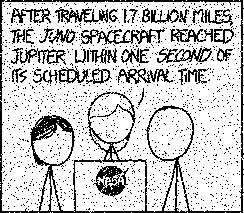
\includegraphics[scale=0.5]{turbo_noisy_60}\\
			Avant d\'ecodage
		\end{minipage}
		\begin{minipage}{.3\textwidth}
			\centering
			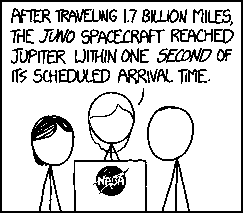
\includegraphics[scale=0.5]{turbo_decoded_60}\\
			Apr\`es d\'ecodage avec turbocodes
		\end{minipage}
		\begin{minipage}{.3\textwidth}
			\centering
			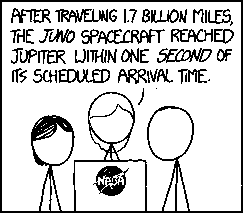
\includegraphics[scale=0.5]{ldpc_basic_decoded_60}\\
			Apr\`es d\'ecodage avec codes LDPC
		\end{minipage}
	\end{minipage}
	\caption{Avec un bruit faible}
	\label{fig:faible}
\end{figure}

\begin{figure}[H]
	\begin{minipage}{\textwidth}
		\begin{minipage}{.3\textwidth}
			\centering
			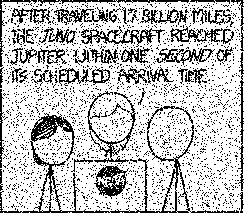
\includegraphics[scale=0.5]{turbo_noisy_80}\\
			Avant d\'ecodage
		\end{minipage}
		\begin{minipage}{.3\textwidth}
			\centering
			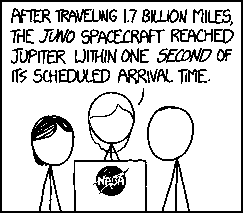
\includegraphics[scale=0.5]{turbo_decoded_80}\\
			Apr\`es d\'ecodage avec turbocodes
		\end{minipage}
		\begin{minipage}{.3\textwidth}
			\centering
			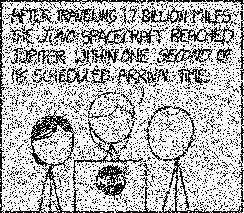
\includegraphics[scale=0.5]{ldpc_basic_decoded_80}\\
			Apr\`es d\'ecodage avec codes LDPC
		\end{minipage}
	\end{minipage}
	\caption{Avec un bruit \'elev\'e}
	\label{fig:eleve}
\end{figure}

\begin{figure}[H]
	\centering
	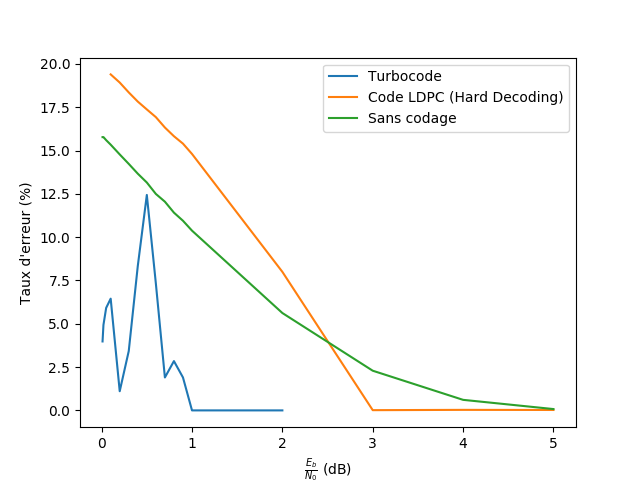
\includegraphics[scale=0.8]{taux_erreur}
	\caption{Taux d'erreur en fonction du SNR}
	\label{fig:taux}
\end{figure}


\section{Calculs pour les turbocodes}
\subsection*{Calcul de $\lambda_k^i(m)$}
\begin{subequations}
\label{eq:1}
On a:
\begin{flalign*}
	\lambda_k^i(m)=\frac{\mathbf{P}(X_k=i,S_k=m,R_1^k,R_{k+1}^N)}{\mathbf{P}(R_1^k,R_{k+1}^N)}=\frac{\mathbf{P}(X_k=i,S_k=m,R_1^k)}{\mathbf{P}(R_1^k)}\frac{\mathbf{P}(R_{k+1}^N|X_k=i,S_k=m,R_1^k)}{\mathbf{P}(R_{k+1}^N|R_1^k)}
\end{flalign*}
Or, puisque $R_{k+1}^N$ n'est pas influenc\'e par $X_k$ ou $R_1^k$, on a :\\
\begin{flalign*}
	\mathbf{P}(R_{k+1}^N|X_k=i,S_k=m,R_1^k)=\mathbf{P}(R_{k+1}^N|S_k=m)
\end{flalign*}
d'o\`u\\
\begin{flalign*}
	\lambda_k^i(m)=\alpha_k^i(m)\beta_k(m)
\end{flalign*}
\end{subequations}


\subsection*{Calcul de $\alpha_k^i(m)$}
\begin{subequations}
\label{eq:2}
On introduit : $\gamma_i(R_k, m', m) = \mathbf{P}(X_k = i, R_k, S_k = m/ S_{k-1} = m')$,\\
\begin{flalign*}
\alpha_k^i(m)=\frac{\mathbf{P}(d_k=i,S_k=m,R_1^{k-1},R_k)}{\mathbf{P}(R_1^{k-1},R_k)}=\frac{\mathbf{P}(d_k=i,S_k=m,R_k|R_1^{k-1})}{\mathbf{P}(R_k|R_1^{k-1})}
\end{flalign*}
Or,\\
\begin{flalign*}
&\mathbf{P}(d_k=i,S_k=m,R_k|R_1^{k-1})=\sum\limits_{m'}\sum\limits_{j=0}^1\mathbf{P}(d_k=i,S_k=m,d_{k-1}=j,S_{k-1}=m',R_k|R_1^{k-1})\\
&=\sum\limits_{m'}\sum\limits_{j=0}^1\mathbf{P}(d_{k-1}=j,S_{k-1}=m'|R_1^{k-1})\times\mathbf{P}(d_k=i,S_k=m,R_k|d_{k-1}=j,S_{k-1}=m',R_1^{k-1})\\
&=\sum\limits_{m'}\sum\limits_{j=0}^1\alpha_{k-1}^j(m')\gamma_i(R_k, m', m)
\end{flalign*}
Ainsi,
\begin{flalign*}
\mathbf{P}(R_k|R_1^{k-1})=\sum\limits_{m'}\sum\limits_{m}\sum\limits_{i=0}^1\sum\limits_{j=0}^1\alpha_{k-1}^j(m')\gamma_i(R_k, m', m)
\end{flalign*}
\end{subequations}

\end{document}